\begin{figure}[htp]
\centering
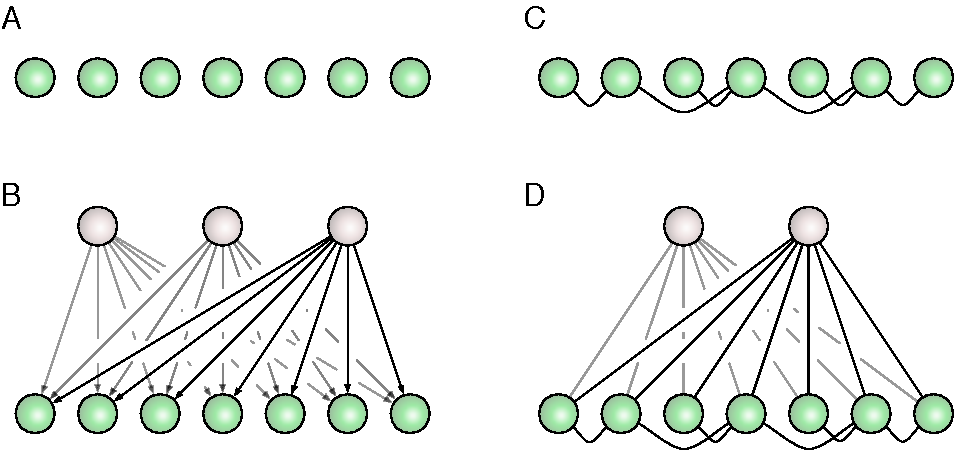
\includegraphics[width=0.5\textwidth]{figures/Figure2.pdf}
\caption{
Graphical models corresponding to the low-dimensional targets of the four regularization schemes used in the paper.
\textbf{A}: A diagonal matrix corresponds to a Gaussian graphical model with no dependencies.
\textbf{B}: In factor analysis, observed nodes are assumed to be influenced by several latent units (``factors") but are otherwise independent.
\textbf{C}: In the Gaussian graphical model (also known as the Gaussian Markov Field), correlations arise from sparse pairwise linear interactions between visible units.
\textbf{D}: In the Gaussian graphical model with latent units, correlations arise  between pairs of nodes
}\label{fig:02}
\end{figure}
